\documentclass[10pt, a4paper]{article}

\usepackage[english]{babel}
\usepackage[utf8]{inputenc}
\usepackage{float}
\usepackage[]{amsmath} 
\usepackage{graphicx}

% Define question and answer command
\newcounter{qcounter}
\newcommand{\q}[2]
{
    \textbf{Q\refstepcounter{qcounter} \arabic{qcounter}: #1} \par
    \textbf{A:} #2
       \par
       \vspace{0.5cm}
} 

\begin{document}

\begin{titlepage}
\centering
{
 \scshape \LARGE 
EL2450 Homework 1
}
\vfill
Andreas Froderberg - 19880730-4577
\par
Martin Favre - 19920130-0010
\end{titlepage}


\q %1
{
    A gain named Tap exists in the Tank 1 model, what is its function?
}
{
    The gain Tap models the bypass tap from the upper tank to the main tank. 
    The value 0 means that it is currently closed. A value of 1 means fully opened.
}
\q  %2
{
    Edit \textit{pid\_design.m} and fill in the transfer functions for the upper
    and lower tank.
}
{
    The figure below shows the result.
    %\begin{figure}[H]
        %\centering
        %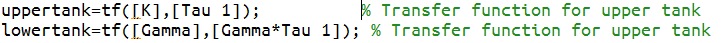
\includegraphics[width=\textwidth]{../images/q2_tfs.png}
    %\end{figure}
}
\q %3
{
    What does the reference signal look like?
}
{
    The signal starts at 40 and recieves a step by 10 at 100 s which sets it to
    50.
}
\q %4
{
    Use the parameter generator to get values and fill in the transfer function
    $F$.
}
{
    Done.
}
\q %5
{
    Use the parameters to get different responses. Which is best?
}
{
    The input parameters and their respecitve system parameters are:
    \begin{table}[H]
        \centering
        \caption{Parameter values and performance.}
        \label{tab:pvals}
        \begin{tabular}{|c|c|c|c|c|c|}
            \hline
            $\chi$ & $\zeta$ & $\omega_0$ & $T_r$ [s] & $M [\%]$ & $T_s$ [s] \\
            \hline
            0.5 & 0.7 & 0.1 & 6.38 & 6.67 & 38.1 \\
            \hline
            0.5 & 0.7 & 0.2 & 3.31 & 22.6 & 18.8 \\
            \hline
            0.5 & 0.8 & 0.2 & 3.19 & 20.9 & 18.4 \\
            \hline
        \end{tabular}
    \end{table}
    The last parameter configuration works best. It is the fastest and even though 
    it has quite significant overshoot, it is still within the given tolerance
    and is thus acceptable.
}
\q %6
{
    What is the cutoff frequency for the open loop system? How was this derived?
}
{
    The open loop system is $G_o=FG$ and the cutoff frequency is the
    frequency when the amplitude gain is 0 dB. Using the bode plots this
    frequency is found to be around $\omega_c=0.35 \text{rad/s}$. This is confirmed by the
    MatLab command \textit{allmargin(Go)} which gives $\omega_c = 0.343 \text{rad/s}$.
}
%%%%%% Part 2 %%%%%%%
\q %7
{
    A ZOH block is placed after the controller. What is the effect?
}
{
    The effect of the system for different sampling times is shown below.
    \begin{figure}[H]
        \centering
        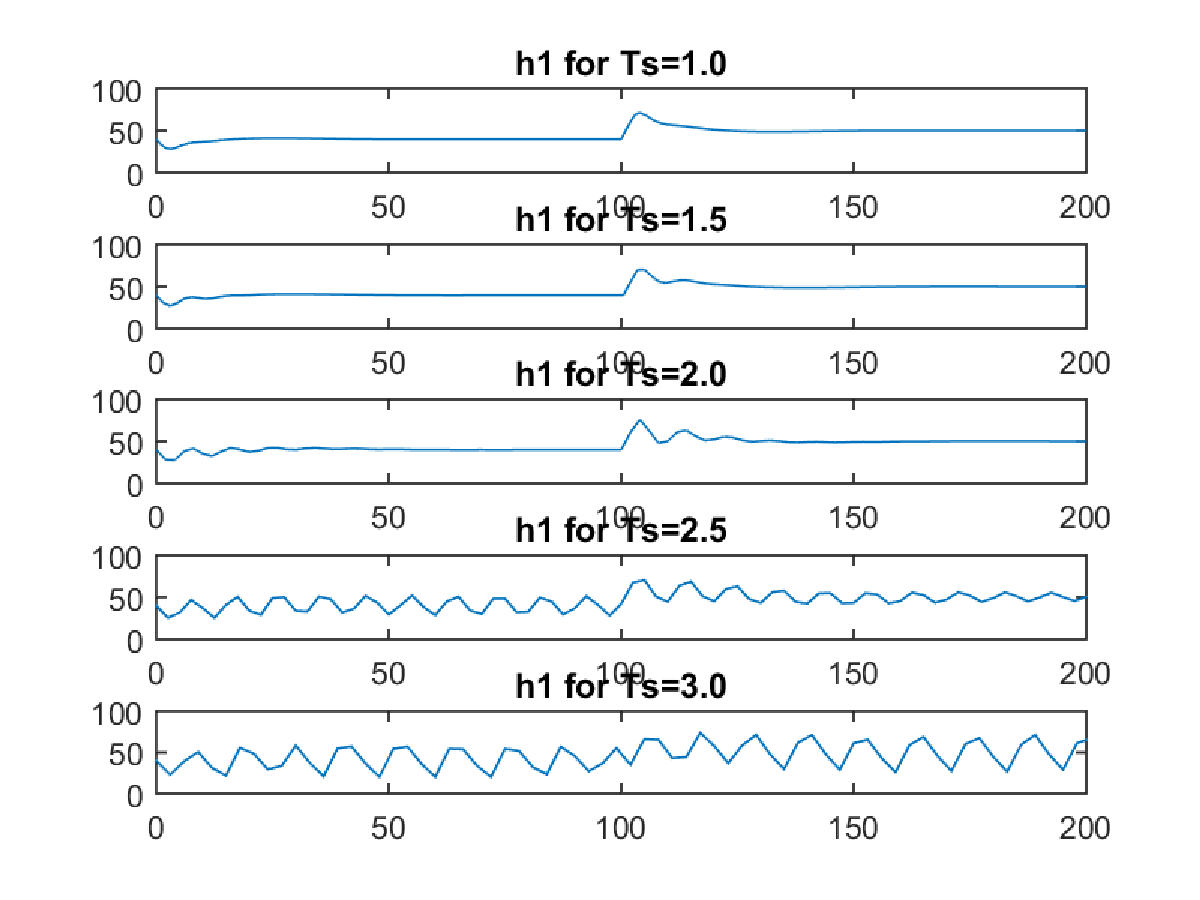
\includegraphics[width=\textwidth]{../Code/images/h1_samplings.png}
        \caption{Upper tank level for different sampling times.}
    \end{figure}
    \begin{figure}[H]
        \centering
        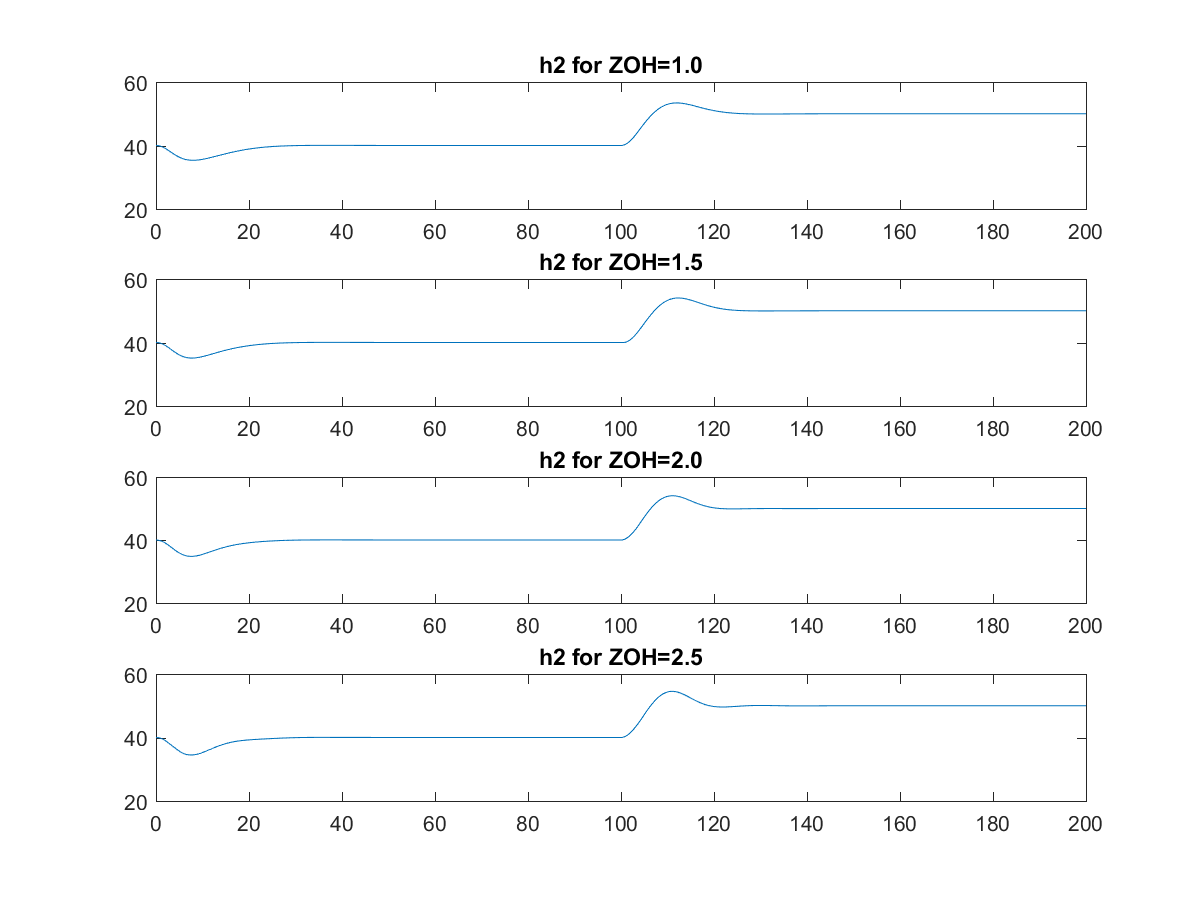
\includegraphics[width=\textwidth]{../Code/images/h2_samplings.png}
        \caption{Lower tank level for different sampling times.}
    \end{figure}
    \begin{figure}[H]
        \centering
        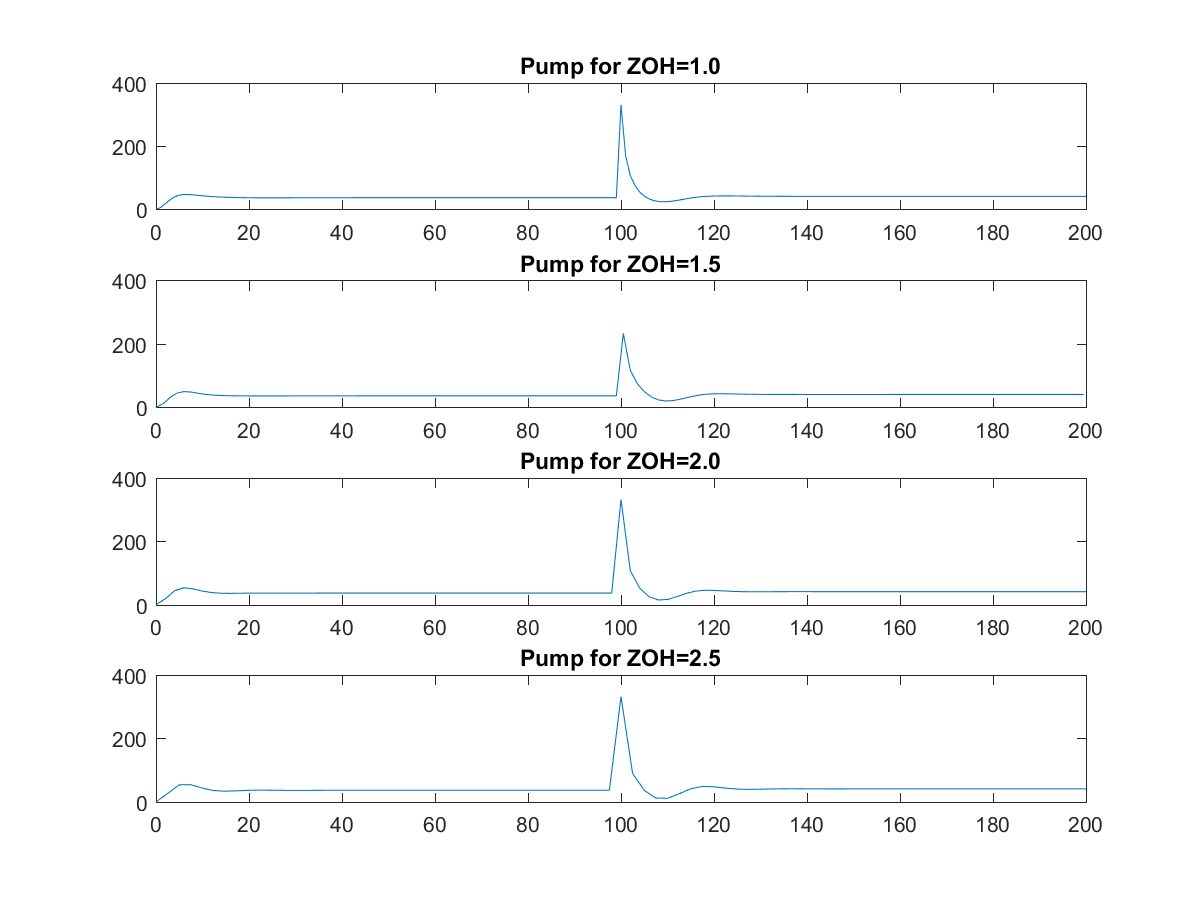
\includegraphics[width=\textwidth]{../Code/images/pump_samplings.png}
        \caption{Pump input for different sampling times.}
    \end{figure}
    From the figures it can be seen that the stabilility and performance of the
    system decreases with higher samplnig time. For a sampling time of about 1
    second, the system is stable and the performance is smooth. At 3 second
    sampling time, it is oscillating and is on the verge of becoming unstable.
}
\q
{
    Discretize the continuous controller into state space form. Replace the
    simulink controller block with this new discrete controller. What differences
    can be seen? 
}
{
    Show images here Andreas. Not of yourself please.

    Comparison shows that ZOH method yields overall better results. This may be due to that the continuous system on which the ZOH method is based is more precise. 
}

\q
{
     What sampling time should be chosen?
}
{
    The crossover frequency of the open-loop system is $\omega_c = 0.34 $ A good sampling frequency is $20\omega_c  = 6.8 rad/s$ \\ 
    This gives a samplingtime of $\frac{2\pi}{20\omega_c} = 0.92 $ seconds
}
\q
{
    How long can the samplingtime be without affecting the performance?
}
{
    With manual checks the maximum samplingtime before the systems starts to strongly oscillate is around 2 to 3 times the recommended sampling time from question 9.
}

\q
{
    Simulate system with samplingtime at 4 seconds and estimate the control performance.
}
{
    The system is asymptotically stable but oscillating.
}
\q
{
    Sample G, make Gd
}
{
    \begin{tabular}{|c|c|}
    \hline 
    $a_1$ &  = 0.092 \\
    \hline
    $a_2$ & = 0.074 \\
    \hline
    \end{tabular}
}
\end{document}
